\documentclass[11pt,oneside]{article}
\usepackage{subfigure}
\usepackage{amsmath}
\usepackage{amssymb}
\usepackage{amsbsy}
\usepackage{mathpazo}
\usepackage{float}
\usepackage{braket}
\setlength{\marginparwidth}{3cm}
\usepackage{todonotes}
\usepackage[spanish]{babel}
\usepackage{graphicx}
\usepackage{listings}
\usepackage{color}
\usepackage{booktabs}
\usepackage{multirow}
\usepackage{ragged2e}
\usepackage{amsmath,blkarray,booktabs,bigstrut}
\usepackage[a4paper, left=2.5cm, right=2.5cm, top=2.5cm, bottom=2.5cm]{geometry}
\usepackage{hyperref}
\usepackage{colortbl}
\usepackage{xcolor}
\usepackage{enumitem}
\usepackage{tcolorbox}
\usepackage{todonotes}

\hypersetup{
    colorlinks=true,
    linkcolor=blue, % Color de los enlaces internos
    filecolor=magenta, % Color de los enlaces a archivos
    urlcolor=blue % Color de los enlaces a URLs
}

\floatstyle{ruled}
\restylefloat{table}

\usepackage{listings}
\usepackage{color}
\lstloadlanguages{csh}

\definecolor{red}{rgb}{0.6,0,0} 
\definecolor{blue}{rgb}{0,0,0.6}
\definecolor{green}{rgb}{0,0.8,0}
\definecolor{cyan}{rgb}{0.0,0.6,0.6}
\definecolor{white}{rgb}{1,1,1}

% Configuración global para todos los recuadros
\tcbset{
    colback=blue!3!white,     % Fondo
    colframe=blue!50!white,   % Borde 
    boxrule=0.5mm,            % Grosor del borde (opcionalmente más delgado)
    title=Información         % Título predeterminado
}

\lstset{
language=csh,
captionpos=b,      % Posición del caption (b: abajo, t: arriba)
basicstyle=\footnotesize\ttfamily,
% numbers=left,
% numberstyle=\tiny,
% numbersep=5pt,
tabsize=2,
extendedchars=true,
% breaklines=true,
% frame=b,
stringstyle=\color{red}\ttfamily,
showspaces=false,
showtabs=false,
% xleftmargin=17pt,
framexleftmargin=17pt,
% framexrightmargin=5pt,
framexbottommargin=4pt,
commentstyle=\color{green},
morecomment=[l]{//}, %use comment-line-style!
morecomment=[s]{/*}{*/}, %for multiline comments
showstringspaces=false,
morekeywords={ abstract, event, new, struct,
as, explicit, null, switch,
base, extern, object, this,
bool, false, operator, throw,
break, finally, out, true,
byte, fixed, override, try,
case, float, params, typeof,
catch, for, private, uint,
char, foreach, protected, ulong,
checked, goto, public, unchecked,
class, if, readonly, unsafe,
const, implicit, ref, ushort,
continue, in, return, using,
decimal, int, sbyte, virtual,
default, interface, sealed, volatile,
delegate, internal, short, void,
do, is, sizeof, while,
double, lock, stackalloc,
else, long, static, get,
enum, namespace, string},
keywordstyle=\color{blue},
identifierstyle=\color{black},
backgroundcolor=\color{white},
inputencoding=utf8,
    literate=%
    {á}{{\'a}}1
    {é}{{\'e}}1
    {í}{{\'i}}1
    {ó}{{\'o}}1
    {ú}{{\'u}}1
    {Á}{{\'A}}1
    {É}{{\'E}}1
    {Í}{{\'I}}1
    {Ó}{{\'O}}1
    {Ú}{{\'U}}1
    {ñ}{{\~n}}1
    {Ñ}{{\~N}}1
    {¡}{{\textexclamdown}}1
    {¿}{{\textquestiondown}}1
}

% Definir tipos personalizados en cian
\lstset{
    classoffset=1,
    morekeywords={
    Program, Console, List, StringBuilder, Array,
    TypeOfTriangle, DayOfWeek,
    NotImplementedException, DivideByZeroException, ArgumentException, 
    ChessPiece,
    BigInt, Fraction, Poly, Set, Book, Genre},
    keywordstyle=\color{cyan},
    classoffset=0,
}

\renewcommand{\lstlistingname}{Figura} % Cambia el prefijo de lstlisting a "Figura"

% Define la variable para controlar la visibilidad de las respuestas
\newif\ifshowanswers

% Define la variable que representa el curso
\def\academicyear{2024 - 2025}

% \showanswerstrue  % Comenta esta línea para ocultar las respuestas

\begin{document}
    \begin{center}
    \begin{large}
    Cp 5 - Arrays\\
    Curso \academicyear\\
    \end{large}
    \begin{figure}[h]
    	\centering
    	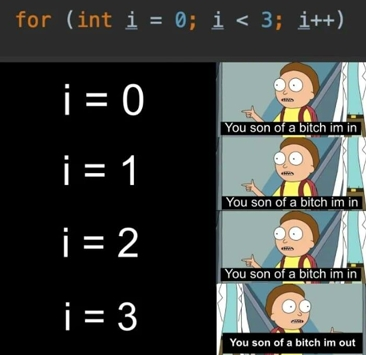
\includegraphics[width=0.5\linewidth]{cp4/loops.jpg}
    \end{figure}
\end{center}

% Intermediate
\section{Invirtiendo}
Implemente un método que reciba como entrada un array \(a\) de elementos y devuelva un nuevo array que contenga los mismos elementos de \(a\) pero en orden inverso.

\subsection*{Entrada:}

Un array \(a = [a_1, a_2, \dots, a_n]\) de \(n\) elementos.

\subsection*{Salida:}

Un array \(b = [b_1, b_2, \dots, b_n]\) tal que \(b_1 = a_n\), \(b_2 = a_{n-1}\), \dots, \(b_n = a_1\).

\subsection*{Ejemplos:}
\begin{itemize}
    \item Entrada: \([1, 2, 3, 4, 5]\) \\
    Salida: \([5, 4, 3, 2, 1]\)
    \item Entrada: \([7, 3, 8, 9]\) \\
    Salida: \([9, 8, 3, 7]\)
    \item Entrada: \([12]\) \\
    Salida: \([12]\)
\end{itemize}

\ifshowanswers
\section*{Respuesta:}
\begin{lstlisting}
public static int[] Reverse(int[] array)
{
    int[] reversed = new int[array.Length];
    
    for (int i = 0; i < array.Length; i++)
    {
        reversed[i] = array[array.Length - 1 - i];
    }
    
    return reversed;
}
\end{lstlisting}
\fi

\section{Filtrando positivos}
\begin{enumerate}[label=\alph*)]
    \item \textbf{Filtrar elementos positivos:} \\
    Implemente un método que reciba un array \(a\) de números enteros y devuelva un nuevo array que contenga únicamente los elementos positivos de \(a\).

    \subsection*{Ejemplos}
    \begin{itemize}
        \item Entrada: \([1, -2, 3, -4, 5]\) \\
        Salida: \([1, 3, 5]\)
        \item Entrada: \([-10, -5, 0, 2, 4]\) \\
        Salida: \([2, 4]\)
        \item Entrada: \([0, -1, -2]\) \\
        Salida: \([]\)
    \end{itemize}

    \item \textbf{Determinar mayoría positiva:} \\
    Implemente un método que determine si la mayoría de los elementos en un array de números enteros son positivos. El método debe devolver \texttt{true} si más de la mitad de los elementos son positivos, y \texttt{false} en caso contrario.

    \subsection*{Ejemplos}
    \begin{itemize}
        \item Entrada: \([1, -2, 3, -4, 5]\) \\
        Salida: \textcolor{blue}{true}  (Ya que 3 de 5 elementos son positivos)
        \item Entrada: \([-1, -2, 4, 5]\) \\
        Salida: \textcolor{blue}{false}  (Ya que solo 2 de 4 elementos son positivos)
        \item Entrada: \([1, -1, 0]\) \\
        Salida: \textcolor{blue}{false}  (Ya que solo 1 de 3 elementos es positivo)
    \end{itemize}
\end{enumerate}
\ifshowanswers
\section*{Respuesta:}
\begin{enumerate}[label=\alph*)]
    \item \textbf{Solución:}
    \begin{lstlisting}
    public static int[] FilterPositive(int[] a)
    {
        // Contar los elementos positivos
        int count = 0;
        
        for (int i = 0; i < a.Length; i++)
        {
            if (a[i] > 0)
            {
                count++;
            }
        }
        
        // Crear un nuevo array para almacenar los elementos positivos
        int[] positiveArray = new int[count];
        
        // Índice para recorrer el array de positivos
        int index 
        
        for (int i = 0; i < a.Length; i++)
        {
            var num = a[i];
            if (num > 0)
            {
                positiveArray[index++] = num;
            }
        }
        
        return positiveArray;
    }
    \end{lstlisting}
    
    Podemos notar que la parte de contar los elementos mayores que 0 se parece mucho a contar los elementos mayores que el promedio. Para evitar duplicar código y mejorar la mantenibilidad, podríamos crear un método que cuente los elementos mayores que un valor \( x \) y reutilizarlo en ambas situaciones.
    
    \begin{lstlisting}
    private static int CountGreaterThan(int[] a, int x)
    {
        int count = 0;
        
        for (int i = 0; i < a.Length; i++)
        {
            if (a[i] > x)
            {
                count++;
            }
        }
        
        return count;
    }
    
    public static int[] FilterPositive(int[] a)
    {
        int count = CountGreaterThan(a, 0);
        int[] positiveArray = new int[count];
        int index = 0;
        
        for (int i = 0; i < a.Length; i++)
        {
            if (a[i] > 0)
            {
                positiveArray[index++] = a[i];
            }
        }
    
        return positiveArray;
    }
    \end{lstlisting}
    \item \textbf{Hint:} Reutiliza el método auxiliar implementado en el inciso anterior.
\end{enumerate}
\fi

\section{Subarray}
Dado un array \(a\) y dos posiciones \(i\) y \(j\) (con \(i \leq j\)), implemente un método que devuelva un nuevo array que contenga el rango de elementos del array original comprendido entre las posiciones \(i\) y \(j\) (inclusive). Es decir, el subarray debe estar formado por los elementos desde el índice \(i\) hasta el índice \(j\) del array original.

Si el array \(a\) tiene \(n\) elementos, y \(a = [a_1, a_2, \dots, a_n]\), el subarray que corresponde al rango \([i..j]\) se obtiene seleccionando los elementos \([a_i, a_{i+1}, \dots, a_j]\).

\subsection*{Ejemplos}
\begin{itemize}
    \item Entrada: \(a = [10, 20, 30, 40, 50]\), \(i = 1\), \(j = 3\) \\
    Salida: \([20, 30, 40]\) \\
    En este caso, el subarray es el que va desde el índice \(1\) (valor \(20\)) hasta el índice \(3\) (valor \(40\)), ambos inclusive.

    \item Entrada: \(a = [1, 2, 3, 4, 5]\), \(i = 0\), \(j = 4\) \\
    Salida: \([1, 2, 3, 4, 5]\) \\
    En este caso, el subarray incluye todos los elementos del array original, ya que \(i = 0\) y \(j = 4\).
    
    \item Entrada: \(a = [7, 8, 9, 10, 11]\), \(i = 3\), \(j = 3\) \\
    Salida: \([10]\) \\
    El subarray contiene solo el elemento en la posición \(3\), que es \(10\), ya que \(i = j = 3\).
\end{itemize}

\section{Operaciones sobre arrays}
\begin{enumerate}[label=\alph*)]
    \item \textbf{Añadir un valor al final del array:} \\
    Implemente un método que reciba un valor \texttt{val} y lo añada al final del array \(a\), devolviendo un nuevo array con el valor añadido.
    
    \subsection*{Ejemplos:}
    \begin{itemize}
        \item Entrada: \(a = [1, 2, 3]\), \texttt{val} = 4 \\
        Salida: \([1, 2, 3, 4]\)
        \item Entrada: \(a = [5, 7, 9]\), \texttt{val} = 10 \\
        Salida: \([5, 7, 9, 10]\)
        \item Entrada: \(a = [1, -50, 2]\), \texttt{val} = 5 \\
        Salida: \([1, -50, 2, 5]\)
    \end{itemize}

    \item \textbf{Insertar un valor en una posición específica:} \\
    Implemente un método que, dado un entero \texttt{pos} y un valor \texttt{val}, inserte el valor \texttt{val} en la posición \texttt{pos} del array \(a\), desplazando los elementos existentes hacia la derecha, y devuelva un nuevo array con el valor insertado.
    
    \subsection*{Ejemplos}
    \begin{itemize}
        \item Entrada: \(a = [1, 3, 4]\), \texttt{pos} = 1, \texttt{val} = 2 \\
        Salida: \([1, 2, 3, 4]\)
        \item Entrada: \(a = [5, 10, 15]\), \texttt{pos} = 2, \texttt{val} = 12 \\
        Salida: \([5, 10, 12, 15]\)
        \item Entrada: \(a = [1, 2, 3, 4]\), \texttt{pos} = 0, \texttt{val} = 0 \\
        Salida: \([0, 1, 2, 3, 4]\)
    \end{itemize}

    \item \textbf{Eliminar un valor en una posición específica:} \\
    Implemente un método que, dado un entero \texttt{pos} referente a una posición del array \(a\), elimine el elemento en esa posición, y devuelva un nuevo array sin ese elemento.
    
    \subsection*{Ejemplos}
    \begin{itemize}
        \item Entrada: \(a = [1, 2, -10, 4]\), \texttt{pos} = 2 \\
        Salida: \([1, 2, 4]\)
        \item Entrada: \(a = [5, 10, 15, 20]\), \texttt{pos} = 1 \\
        Salida: \([5, 15, 20]\)
        \item Entrada: \(a = [8, 6, 7]\), \texttt{pos} = 0 \\
        Salida: \([6, 7]\)
    \end{itemize}

    \item \textbf{Eliminar la primera ocurrencia de un valor:} \\
    Implemente un método que, dado un valor \texttt{val}, elimine la primera ocurrencia de dicho valor en el array \(a\), y devuelva un nuevo array sin ese valor.
    
    \subsection*{Ejemplos}
    \begin{itemize}
        \item Entrada: \(a = [1, 2, 3, 2, 4]\), \texttt{val} = 2 \\
        Salida: \([1, 3, 2, 4]\)
        \item Entrada: \(a = [5, 5, 10, 15]\), \texttt{val} = 5 \\
        Salida: \([10, 15, 5]\)
        \item Entrada: \(a = [3, 2, 3, 4, 5]\), \texttt{val} = 3 \\
        Salida: \([2, 3, 4, 5]\)
    \end{itemize}
\end{enumerate}
\ifshowanswers
\section*{Respuesta:}
\begin{enumerate}[label=\alph*)]
    \item \textbf{Solución:}
    \begin{lstlisting}
    public static int[] Add(int[] array, int val)
    {
        int[] newArray = new int[array.Length + 1];
        
        for (int i = 0; i < array.Length; i++)
        {
            newArray[i] = array[i];
        }
        
        newArray[array.Length] = val;
        
        return newArray;
    }
    \end{lstlisting}
    \item \textbf{Solución:}
    \begin{lstlisting}
    public static int[] Insert(int[] array, int pos, int val)
    {
        int[] newArray = new int[array.Length + 1];
        
        for (int i = 0; i < pos; i++)
        {
            newArray[i] = array[i];
        }
        
        newArray[pos] = val;
        
        for (int i = pos; i < array.Length; i++)
        {
            newArray[i + 1] = array[i];
        }
        
        return newArray;
    }
    \end{lstlisting}
    \item \textbf{Solución:}
    \begin{lstlisting}
    public static int[] RemoveAt(int[] array, int pos)
    {
        int[] newArray = new int[array.Length - 1];
        
        for (int i = 0; i < pos; i++)
        {
            newArray[i] = array[i];
        }
        
        for (int i = pos + 1; i < array.Length; i++)
        {
            newArray[i - 1] = array[i];
        }
        
        return newArray;
    }
    \end{lstlisting}
\end{enumerate}

\fi

% Advanced
\section{Rotando arrays}
Implemente un método que reciba un array \(a\) y un entero \(veces\) y rote los elementos del array tantas veces como indique el parámetro \(veces\). Si \(veces\) es positivo, rota los elementos a la derecha; si es negativo, rota los elementos a la izquierda. Si \(veces\) es 0, el array no se %ifica.


\subsection*{Ejemplos}

\begin{itemize}
    \item Entrada: \(a = [25, 40, 17, 83, 9]\), \(veces = 2\)\\
    Salida: \([83, 9, 25, 40, 17]\)\\
    % Explicación: Al rotar el array dos veces hacia la derecha, los últimos dos elementos (\(83, 9\)) se mueven al inicio, mientras que los demás se desplazan hacia la derecha.

    \item Entrada: \(a = [25, 40, 17, 83, 9]\), \(veces = -2\)\\
    Salida: \([17, 83, 9, 25, 40]\)\\
    % Explicación: Al rotar el array dos veces hacia la izquierda, los dos primeros elementos (\(25, 40\)) se mueven al final, mientras que los demás se desplazan hacia la izquierda.

    \item Entrada: \(a = [1, 2, 3, 4, 5]\), \(veces = 0\)\\
    Salida: \([1, 2, 3, 4, 5]\)\\
    % Explicación: No se realiza ninguna rotación, ya que \(veces = 0\), por lo que el array permanece sin cambios.

    \item Entrada: \(a = [7, 14, 21]\), \(veces = 7\)\\
    Salida: \([21, 7, 14]\)\\
    Explicación: Rotar \(veces = 7\) es equivalente a rotar \(veces = 1\) (ya que \(7 \% 3 = 1\), donde \(3\) es el tamaño del array). 
    % Esto mueve el último elemento (\(21\)) al inicio y desplaza los demás hacia la derecha.

    \item Entrada: \(a = [5, 10, 15, 20]\), \(veces = -5\)\\
    Salida: \([10, 15, 20, 5]\)\\
    Explicación: Rotar \(veces = -5\) es equivalente a rotar \(veces = -1\) (ya que \(-5 \% 4 = -1\), donde \(4\) es el tamaño del array). 
    % Esto mueve el primer elemento (\(5\)) al final y desplaza los demás hacia la izquierda.
\end{itemize}

\ifshowanswers
\section*{Respuesta:}
Imaginemos un array de tamaño $n = 5$. Nos podemos dar cuenta de que el resultado de rotar 3 veces es equivalente al de rotar 8, o al de rotar 13. Esto se debe a que al rotar el array tantas veces como su tamaño, el array vuelve a su estado original. Por lo tanto, al rotar más de $n$ veces, estamos realizando rotaciones adicionales que no cambian el resultado final. Al aplicar la operación módulo (\%), obtenemos el menor número de rotaciones necesarias para lograr el mismo resultado.

Veamos qué pasa con las rotaciones negativas. Podemos darnos cuenta de que, en nuestro array de 5 elementos, rotar -2 veces es equivalente a rotar -7, o -22 veces, pero también es equivalente a rotar 3 veces. 

Como la operación módulo (\%) en C\# da como resultado números en el rango \([-(k-1), k-1]\). Si el resultado es menor que 0, podemos sumarle \( k \) para obtener un valor positivo. Por ejemplo:

\[
-22 \% 5 = -2
\]
\[
-2 + 5 = 3
\]

De esta manera, siempre obtenemos la mínima cantidad de veces que debemos rotar a la derecha para obtener el mismo resultado.

Primero podemos resolver el problema de rotar una vez a la derecha. La rotación una vez a la derecha implica mover cada elemento del array una posición hacia adelante, y mover el último elemento al primer lugar.

\begin{lstlisting}
private static void RotateOnce(int[] array)
{
    int lastElement = array[^1]; // Notación de C# equivalente a array[array.Length - 1]
    
    for (int i = array.Length - 1; i > 0; i--)
    {
        array[i] = array[i - 1];
    }
    
    array[0] = lastElement;
}
\end{lstlisting}

Luego, podemos llamar $k$ veces a este método para lograr la rotación deseada:

\begin{lstlisting}
public static void Rotate(int[] array, int times)
{
    if (array.Length == 0)
        return;

    // Normalizar times para que esté dentro del rango de la longitud del array
    times %= array.Length;
    
    if (times < 0)
        times += array.Length;
        
    for (int i = 0; i < times; i++)
    {
        RotateOnce(array);
    }
}
\end{lstlisting}

En general, podemos determinar la posición final de cada elemento en la rotación, ya que al mover cada elemento $k$ posiciones a la derecha, este se ubicará en una posición específica calculable dentro del array. 

\begin{lstlisting}
public static void Rotate(int[] array, int times)
{
    if (array.Length == 0)
            return;
            
    // Normalizar times para que esté dentro del rango de la longitud del array
    times %= array.Length;

    if (times < 0)
        times += array.Length;
        
    // Copiar los elementos del array original en el array temporal
    // en sus nuevas posiciones rotadas
    int[] temp = new int[array.Length];

    for (int i = 0; i < array.Length; i++)
    {
        temp[(i + times) % array.Length] = array[i];
    }

    // Copiar los elementos ya rotados al array original
    for (int i = 0; i < length; i++)
    {
        array[i] = temp[i];
    }
}
\end{lstlisting}

Podemos solucionar el problema sin usar un array auxiliar. Notemos que siempre sabemos en qué posición terminará el elemento, pero no podemos moverlo y ya, pues sobreescribiríamos el elemento que estaba en la posición a donde lo estamos moviendo.

Supongamos que tenemos el array $[1, 2, 3, 4, 5, 6]$, de tamaño $n = 6$ y queremos rotar $k = 4$ veces. Comenzamos en la posición 0  y sigamos estos pasos:
\begin{enumerate}
    \item El valor en la posición 0 (valor 1) se mueve a la posición 4. 
    \[[1, 2, 3, 4, 1, 6]\]
    \item El valor que estaba en la posición 4 (valor 5) se mueve a la posición 2. 
    \[[1, 2, 5, 4, 1, 6]\]
    \item El valor que estaba en la posición 2 (valor 3) se mueve a la posición 0 (la posición de inicio). 
    \[[3, 2, 5, 4, 1, 6]\]
\end{enumerate}

Notemos que ya hemos cubierto los índices [0, 2, 4], o sea, los valores que están en estos índices están correctamente rotados.

Ahora hagamos lo mismo comenzando en la posición 1 en el array reultante $[3, 2, 5, 4, 1, 6]$:
\begin{enumerate}
    \item El valor en la posición 1 (valor 2) se mueve a la posición 5. 
    \[[3, 2, 5, 4, 1, 2]\]
    \item El valor que estaba en la posición 5 (valor 6) se mueve a la posición 3. 
    \[[3, 2, 5, 6, 1, 2]\]
    \item El valor que estaba en la posición 3 (valor 4) se mueve a la posición 1 (la posición de inicio). 
    \[[3, 4, 5, 6, 1, 2]\]
\end{enumerate}

Notemos que ya hemos cubierto correctamente todos los índices del array, por tanto ya quedó completamente rotado.

El siguiente código rota correctamente un array $k$ veces:

\begin{lstlisting}
public static void Rotate(int[] array, int times)
{
    if (array.Length == 0)
        return;

    // Normalizar times para que esté dentro del rango de la longitud del array
    times %= array.Length;
    if (times < 0)
        times += array.Length;
        
    int startIndex = 0;
    int totalCount = 0;
    
    while (totalCount < array.Length)
    {
        totalCount += RotateCycle(array, times, startIndex);
    }
}
    
// Ejecuta un ciclo de rotaciones comenzando desde 'startIndex'
// y devuelve la cantidad de elementos que fueron rotados en ese ciclo
public static int RotateCycle(int[] array, int times, int startIndex)
{
    int currentIndex = startIndex;
    int currentElement = array[startIndex];
    int count = 0;
    do
    {
        int nextIndex = (currentIndex + times) % array.Length;
        
        int temp = array[nextIndex];
        array[nextIndex] = currentElement;
        currentElement = temp;
        
        currentIndex = nextIndex;
        count++;
    } while (currentIndex != startIndex);
    return count;
}
\end{lstlisting}


\fi

\section{Invirtiendo bloques}
Implemente un método que, dado un número entero \(k\), invierta cada subarray de longitud \(k\) dentro del array \(a\), comenzando desde posiciones múltiplo de \(k\). Si el último segmento tiene menos de \(k\) elementos, también debe invertirse.

\subsection*{Ejemplos}

\begin{itemize}
    \item \textbf{Entrada:} \(a = [1, 2, 3, 4, 5, 6, 7, 8, 9, 10], \, k = 3\)\\
    \textbf{Salida:} \([3, 2, 1, 6, 5, 4, 9, 8, 7, 10]\)\\
    \textbf{Explicación:} 
    \begin{itemize}
        \item El subarray \([1, 2, 3]\) se invierte en \([3, 2, 1]\).
        \item El subarray \([4, 5, 6]\) se invierte en \([6, 5, 4]\).
        \item El subarray \([7, 8, 9]\) se invierte en \([9, 8, 7]\).
        \item El último elemento \(10\), aunque no forma un subarray completo, también se invierte, resultando en sí mismo.
    \end{itemize}

    \item \textbf{Entrada:} \(a = [1, 2, 3, 4, 5, 6, 7], \, k = 4\)\\
    \textbf{Salida:} \([4, 3, 2, 1, 7, 6, 5]\)\\
    \textbf{Explicación:}
    \begin{itemize}
        \item El subarray \([1, 2, 3, 4]\) se invierte en \([4, 3, 2, 1]\).
        \item El subarray incompleto \([5, 6, 7]\) se invierte en \([7, 6, 5]\).
    \end{itemize}

    \item \textbf{Entrada:} \(a = [7, 14, 21, 28, 35, 42], \, k = 6\)\\
    \textbf{Salida:} \([42, 35, 28, 21, 14, 7]\)\\
    \textbf{Explicación:}
    \begin{itemize}
        \item Todo el array \([7, 14, 21, 28, 35, 42]\) forma un único subarray que se invierte completamente, resultando en \([42, 35, 28, 21, 14, 7]\).
    \end{itemize}

    \item \textbf{Entrada:} \(a = [1, 2, 3], \, k = 1\)\\
    \textbf{Salida:} \([1, 2, 3]\)\\
    \textbf{Explicación:}
    \begin{itemize}
        \item Como \(k = 1\), cada subarray tiene un solo elemento, por lo que no hay cambios.
    \end{itemize}
\end{itemize}


\section{Mezcla ordenada}
Implemente un método que, dados dos arrays ordenados \(a\) y \(b\), devuelva un nuevo array que sea la mezcla ordenada de estos. Los elementos repetidos deben incluirse tantas veces como aparezcan en los arrays originales.

\subsection*{Ejemplos}

\begin{itemize}
    \item Entrada: \(a = [23, 40, 83], \, b = [5, 17, 23, 24, 51]\)\\
    Salida: \([5, 17, 23, 23, 24, 40, 51, 83]\)

    \item Entrada: \(a = [1, 3, 5, 7], \, b = [2, 4, 6, 8]\)\\
    Salida: \([1, 2, 3, 4, 5, 6, 7, 8]\)

    \item Entrada: \(a = [10, 20, 30], \, b = []\)\\
    Salida: \([10, 20, 30]\)

    \item Entrada: \(a = [1, 1, 3], \, b = [1, 2, 2, 3]\)\\
    Salida: \([1, 1, 1, 2, 2, 3, 3]\)
\end{itemize}

\ifshowanswers
\section*{Respuesta:}
\begin{lstlisting}
public static int[] MergeSortedArrays(int[] a, int[] b)
{
    int[] result = new int[a.Length + b.Length];

    // Inicializa los índices para recorrer los arrays 'a', 'b' y 'result'
    int i = 0, j = 0, k = 0;

    // Itera mientras haya elementos en ambos arrays 'a' y 'b'
    while (i < a.Length && j < b.Length)
    {
        // Si el elemento actual de 'a' es menor que el de 'b'
        if (a[i] < b[j])
        {
            // Copia el elemento de 'a' en 'result' y avanza los índices 'i' y 'k'
            result[k++] = a[i++];
        }
        else
        {
            // Copia el elemento de 'b' en 'result' y avanza los índices 'j' y 'k'
            result[k++] = b[j++];
        }
    }

    // Copia los elementos restantes de 'a' en 'result', si los hay
    while (i < a.Length)
    {
        result[k++] = a[i++];
    }

    // Copia los elementos restantes de 'b' en 'result', si los hay
    while (j < b.Length)
    {
        result[k++] = b[j++];
    }

    return result;
}
\end{lstlisting}
\fi

\section{Ordenando}
Implemente un método que reciba un array de enteros \(a\) y devuelva un nuevo array que contenga los mismos elementos de \(a\) pero ordenados de menor a mayor.

\subsection*{Ejemplos}

\begin{itemize}
    \item Entrada: \(a = [5, 2, 9, 1, 5, 6]\)\\
    Salida: \([1, 2, 5, 5, 6, 9]\)\\

    \item Entrada: \(a = [10, -5, 7, 3, 0]\)\\
    Salida: \([-5, 0, 3, 7, 10]\)\\

    \item Entrada: \(a = [1, 2, 3, 4]\)\\
    Salida: \([1, 2, 3, 4]\)\\

    \item Entrada: \(a = [42]\)\\
    Salida: \([42]\)\\

    \item Entrada: \(a = []\)\\
    Salida: \([]\)\\
\end{itemize}


\section{Operaciones con conjuntos}
Dado dos conjuntos \( A \) y \( B \), representados mediante arreglos (arrays), implementa métodos para realizar las siguientes operaciones fundamentales de teoría de conjuntos. Cada método debe devolver un nuevo arreglo que represente el resultado de la operación, asegurándote de que los elementos no se repitan:
    
\begin{enumerate}
    \item \( A \cap B \): Devuelve los elementos que están en \( A \) \textbf{y} en \( B \) (intersección).
    \item \( A \cup B \): Devuelve los elementos que están en \( A \) \textbf{o} en \( B \) (unión).
    \item \( A \setminus B \): Devuelve los elementos que están en \( A \) pero \textbf{no} en \( B \) (diferencia).
    \item \( A \, \Delta \, B \): Devuelve los elementos que están en \( A \) pero no en \( B \), \textbf{más} los elementos que están en \( B \) pero no en \( A \) (diferencia simétrica).
\end{enumerate}
\subsection*{Ejemplos}
\begin{itemize}
    \item Entrada: \( A = [1, 2, 3, 4] \), \( B = [3, 4, 5, 6] \)
    \begin{enumerate}
        \item \( A \cap B \): Intersección\\
        Salida: \([3, 4]\)

        \item \( A \cup B \): Unión\\
        Salida: \([1, 2, 3, 4, 5, 6]\)

        \item \( A \setminus B \): Diferencia\\
        Salida: \([1, 2]\)

        \item \( A \, \Delta \, B \): Diferencia simétrica\\
        Salida: \([1, 2, 5, 6]\)\\
        Explicación: Los elementos exclusivos de cada conjunto son \(1, 2\) (de \(A\)) y \(5, 6\) (de \(B\)).
    \end{enumerate}

    \item Entrada: \( A = [10, 20, 30] \), \( B = [30, 40, 50] \)
    \begin{enumerate}
        \item \( A \cap B \): Intersección\\
        Salida: \([30]\)

        \item \( A \cup B \): Unión\\
        Salida: \([10, 20, 30, 40, 50]\)

        \item \( A \setminus B \): Diferencia\\
        Salida: \([10, 20]\)

        \item \( A \, \Delta \, B \): Diferencia simétrica\\
        Salida: \([10, 20, 40, 50]\)\\
        Explicación: Los elementos exclusivos son \(10, 20\) (de \(A\)) y \(40, 50\) (de \(B\)).
    \end{enumerate}

    \item Entrada: \( A = [1, 2, 3] \), \( B = [] \)
    \begin{enumerate}
        \item \( A \cap B \): Intersección\\
        Salida: \([]\)

        \item \( A \cup B \): Unión\\
        Salida: \([1, 2, 3]\)

        \item \( A \setminus B \): Diferencia\\
        Salida: \([1, 2, 3]\)

        \item \( A \, \Delta \, B \): Diferencia simétrica\\
        Salida: \([1, 2, 3]\)
    \end{enumerate}
\end{itemize}
\end{document}
